\section{Results and Discussion}
\label{sec:results_discussion}

\subsection{Primary Comparison}

Table~\ref{tab:primary_results} reports the three systems on the common locked
test cohort.

\begin{table}[t]
    \centering
    \caption{Four-class internal-test performance. Bold indicates the highest
    point estimate in each column.}
    \label{tab:primary_results}
    \footnotesize
    \setlength{\tabcolsep}{2.5pt}
    \begin{tabular}{lcccc}
        \toprule
        System & Acc. & BAcc. & M-F1 & W-F1 \\
        \midrule
        DenseNet-121
        & \textbf{0.7914}
        & 0.6168
        & \textbf{0.6351}
        & \textbf{0.7862} \\

        EfficientNet-B0
        & 0.7421
        & \textbf{0.6503}
        & 0.6192
        & 0.7526 \\

        Hierarchy
        & 0.7402
        & 0.6312
        & 0.6054
        & 0.7503 \\
        \bottomrule
    \end{tabular}
\end{table}

DenseNet-121 exceeded flat EfficientNet-B0 by 0.0493 accuracy, 0.0159
macro-F1, and 0.0336 weighted-F1, but its balanced accuracy was lower by
0.0335. Relative to the hierarchy, its accuracy and macro-F1 were higher by
0.0513 and 0.0297, respectively, while balanced accuracy was lower by 0.0144.

Thus, the descriptive ranking depends on the evaluation metric. DenseNet-121
had the strongest aggregate point estimates, whereas EfficientNet-B0 had the
highest average recall across classes. Paired analyses supported DenseNet-121's accuracy and weighted-F1 gains
over both comparators. Its macro-F1 gain was supported only against the
hierarchy, while its balanced accuracy was significantly lower than that
of flat EfficientNet-B0.

\subsection{Class-Specific Behaviour}

\begin{table}[t]
\caption{Class-Specific Performance on the Locked Internal Test Set}
\label{tab:per_class_comparison}
\centering
\footnotesize
\setlength{\tabcolsep}{4pt}
\begin{tabular}{llcc}
\hline
System & Class & Recall & F1 \\
\hline
DenseNet-121
    & Non-malignant & 0.8912 & 0.8678 \\
    & Melanoma      & 0.5634 & 0.6025 \\
    & BCC           & 0.7149 & 0.7265 \\
    & SCC           & 0.2979 & 0.3436 \\
\hline
EfficientNet-B0
    & Non-malignant & 0.7473 & 0.8218 \\
    & Melanoma      & 0.7537 & 0.6094 \\
    & BCC           & 0.7811 & 0.6885 \\
    & SCC           & 0.3191 & 0.3571 \\
\hline
Hierarchy
    & Non-malignant & 0.7794 & 0.8266 \\
    & Melanoma      & 0.6829 & 0.5784 \\
    & BCC           & 0.7008 & 0.6987 \\
    & SCC           & 0.3617 & 0.3178 \\
\hline
\end{tabular}
\end{table}

Table~\ref{tab:per_class_comparison} reports recall and F1 for all three
systems, while Fig.~\ref{fig:confusion_comparison} provides a visual
comparison of the backbone-matched flat EfficientNet-B0 model and the
conditional hierarchy.

\begin{figure*}[t]
    \centering
    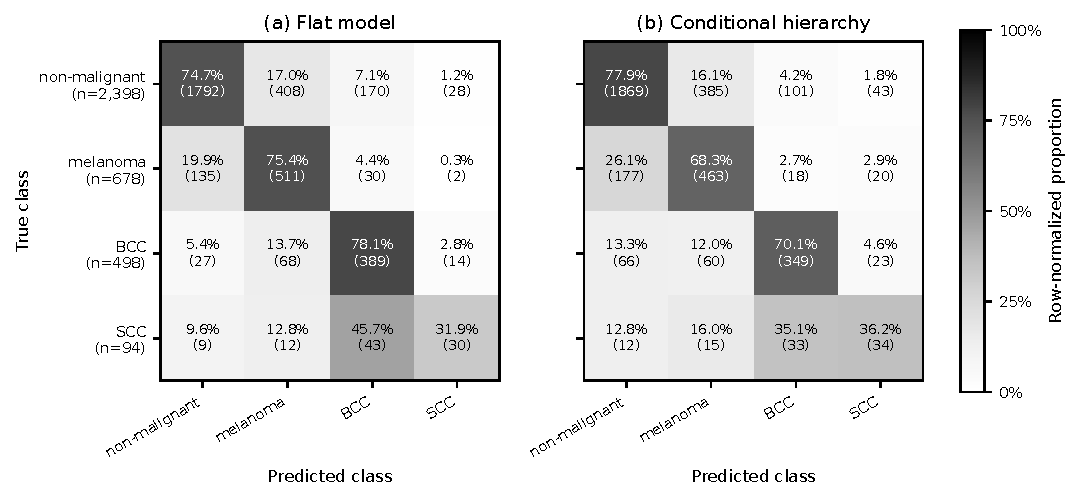
\includegraphics[width=0.94\textwidth]
    {figures/figure02_confusion_matrix_comparison.pdf}
    \caption{Row-normalised confusion matrices for flat EfficientNet-B0 and
    the predicted-gate hierarchy on the common locked test cohort. Counts are
    shown in parentheses. DenseNet-121 is not included in this figure.}
    \label{fig:confusion_comparison}
\end{figure*}

Flat EfficientNet-B0 achieved recalls of 74.7\%, 75.4\%, 78.1\%, and 31.9\%
for non-malignant, melanoma, BCC, and SCC. The hierarchy increased
non-malignant and SCC recall to 77.9\% and 36.2\%, but melanoma and BCC recall
fell to 68.3\% and 70.1\%. Conditional decomposition therefore did not produce
a uniform class-level improvement.

DenseNet-121 achieved recalls of 89.1\%, 56.3\%, 71.5\%, and 29.8\% for the
same classes. Its high majority-class recall contributed strongly to its
aggregate accuracy, while melanoma and SCC remained weak. Only 28 of 94 SCC
images were correctly classified, giving SCC recall 0.2979 and F1 0.3436.
The alternative backbone therefore did not resolve rare-class sensitivity.

\subsection{Paired Model Comparisons}

The paired bootstrap estimated the macro-F1 difference (flat minus hierarchy)
as 0.013855, with 95\% confidence interval
$[-0.014255,\,0.041963]$. The corresponding accuracy difference was 0.001908
with interval $[-0.011996,\,0.015812]$.

The paired correctness table contained 354 images correctly classified only
by the flat model and 347 correctly classified only by the hierarchy. Exact
two-sided McNemar testing yielded $p=0.820742$. The analysis therefore did not
detect a statistically significant difference between the EfficientNet-B0
systems. This does not establish equivalence, non-inferiority, or identical
performance.

Additional paired analyses compared DenseNet-121 with both EfficientNet-B0
systems. Relative to flat EfficientNet-B0, DenseNet-121 increased accuracy
by 0.0493 (95\% CI [0.0352, 0.0632]) and weighted-F1 by 0.0336
([0.0198, 0.0471]), but reduced balanced accuracy by 0.0335
([-0.0636, -0.0037]). Its macro-F1 difference of 0.0159 was inconclusive
([-0.0148, 0.0463]). Relative to the hierarchy, DenseNet-121 increased
accuracy by 0.0513 ([0.0371, 0.0654]), weighted-F1 by 0.0358
([0.0221, 0.0495]), and macro-F1 by 0.0297 ([0.0003, 0.0588]).
The balanced-accuracy difference of $-0.0144$ was inconclusive
([-0.0449, 0.0169]). Exact McNemar tests also detected differences in
paired correctness against flat EfficientNet-B0 ($p=7.01\times10^{-11}$)
and the hierarchy ($p=8.15\times10^{-12}$).

\subsection{Routing-Error Decomposition}

\begin{table}[t]
    \centering
    \caption{Conditional-hierarchy routing analysis.}
    \label{tab:routing_results}
    \footnotesize
    \setlength{\tabcolsep}{3.5pt}
    \begin{tabular}{lr}
        \toprule
        Quantity & Result \\
        \midrule
        Predicted-gate macro-F1 & 0.605367 \\
        Oracle-routing macro-F1 & 0.793656 \\
        Routing-associated loss & 0.188289 \\
        \midrule
        Malignant blocked at Stage~1
        & $255/1{,}270$ (20.079\%) \\
        Non-malignant sent to Stage~2
        & $529/2{,}398$ (22.060\%) \\
        Wrong subtype after correct route
        & $169/1{,}015$ (16.650\%) \\
        \bottomrule
    \end{tabular}
\end{table}

Oracle routing increased macro-F1 from 0.6054 to 0.7937. Among 1,270
malignant images, 255 were blocked before subtype classification. Conversely,
529 non-malignant images were sent to a classifier restricted to malignant
outputs. These counts correspond to a malignant-class sensitivity of 79.921\%
and a non-malignant specificity of 77.940\% at the Stage 1 gate. Among the 1,015 malignant images correctly routed to Stage~2, 169
received the wrong subtype.

Both Stage~1 routing-error rates exceeded the subtype-error rate among
correctly routed malignant images. Together with the 0.1883 macro-F1 gap, these findings indicate that Stage 1
routing errors were a substantial contributor to endpoint performance loss
in the implemented hierarchy. The oracle score remains a diagnostic upper bound: it uses
ground-truth routing and does not predict what a practically improved gate
would achieve.

\subsection{Standalone T-Category Feasibility}

The validation-selected weighted-cross-entropy model obtained test macro-F1
0.275611 and balanced accuracy 0.386039 on the 127-image T-category test
partition. T2 and T4 recalls were both zero, with supports of seven and one.
The aggregate scores therefore conceal complete failure on the scarcest
categories.

This experiment provides standalone feasibility evidence under severe label
scarcity. It does not constitute clinically useful staging, deployable
melanoma assessment, or an integrated three-stage result.

\subsection{Limitations}

The study used one random seed and one internal ISIC-derived cohort, limiting
the generalisability of the observed differences. The split controlled
available lesion identifiers and exact duplicates, but patient-independent
separation could not be guaranteed because patient identifiers were
unavailable and 2,084 images lacked lesion identifiers. SCC had only 94 test
images, and the standalone T-category task had still smaller rare classes.

No external evaluation, calibration study, explainability experiment, or
skin-tone fairness analysis was completed. Direct numerical comparison with
studies using different classes, datasets, or splitting procedures would
therefore be misleading. The evidence supports an internal routing-error
analysis, not clinical validation, external generalisation, or deployment
readiness.
